\documentclass{article}
% \documentclass[12pts]{article}


% ---------------- Packages ----------------
\usepackage[english]{babel}
\usepackage[letterpaper, top=2.5cm, bottom=2.5cm, left=3cm, right=3cm]{geometry}
\usepackage{graphicx} % for figures
\usepackage{setspace} % for spacing
\usepackage[colorlinks=true, allcolors=blue]{hyperref} % for hyperlinks
\usepackage{amsmath, amssymb} % math symbols
\usepackage{float} % for figure placement
\usepackage{caption} % customize captions
\usepackage{booktabs} % nice tables
\usepackage{appendix} % for appendices
\usepackage[justification=centering]{caption}
\usepackage[utf8]{inputenc}




\geometry{margin=1in}

\setlength{\parskip}{0.5em} % spacing between paragraphs
\setlength{\parindent}{0em} % no indentation



\begin{document}

% ---------------- Title Page ----------------
\begin{titlepage}
    \centering
    
    
    
    {\Huge \textbf{Carleton University}}\\[1.5cm]
    
    \vfill % pushes the next block toward the vertical middle
    
    % Title
    {\LARGE \textbf{Course Project: SCARA Robot Report}}\\[1.5cm]
    
    % Course info
    {\Large MECH 4503A: An Introduction to Robotics}\\[0.5cm]
    
    \vfill % pushes the rest (name/date) toward the bottom
    
    
    % Author info
    \vfill
    \begin{flushleft}
    \textbf{Name:} Rami Mrad\\
    \textbf{Student ID:} 101237780\\
    \textbf{Professor:} J.Z. Sasiadek\\
    \end{flushleft}
    
    \vfill

    % Date
    {\Large March 25, 2026}
    
\end{titlepage}
% ---------------- End Title Page ----------------

% Title Page, Introduction, Prelab, Materials and Setup, Procedure, Results, Discussion, Conclusion, References, and Appendices



% \begin{figure}[H]
%     \centering
%     \includegraphics[width=0.85\textwidth]{Part1-spectrum.png}
%     \caption{Spectrum of aliased signal}
%     \label{fig:Part1-spectrum.png}
% \end{figure}


% \begin{equation}
% F_{gen} = \frac{F_s}{2^N} \Delta_{ACC}
% \end{equation}

% ---------------- Sections 1----------------
\section{Introduction}





% ---------------- Section 2 ----------------
\section{SCARA Robot Architecture}

\subsection{Mechanical Configuration}
The canonical 4-DOF SCARA robot (Figure \ref{fig:SCARA_config.png}) consists of a fixed base, two horizontal revolute links of lengths $a_1$ and $a_2$, a vertical prismatic joint, and a final revolute wrist joint. Table 1 summarises the joint types and their physical roles [1][2].

\begin{table}[h!]
\centering

\begin{tabular}{lllll}
\toprule
Joint & Type & Symbol & Motion & Role \\
\midrule
1 & Revolute & $\theta_1$ & Rotation about $Z_0$ & Shoulder rotation in XY plane \\
2 & Revolute & $\theta_2$ & Rotation about $Z_1$ & Elbow rotation in XY plane \\
3 & Prismatic & $d_3$ & Translation along $Z_2$ & Vertical (Z) positioning \\
4 & Revolute & $\theta_4$ & Rotation about $Z_3$ & End-effector spin / tool orientation \\
\bottomrule
\end{tabular}
\caption{SCARA joint summary [1][2].}
\end{table}
\begin{figure}[H]
    \centering
    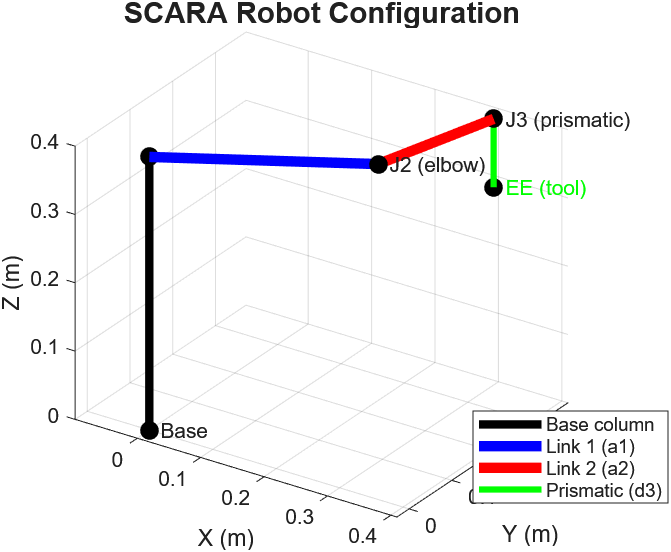
\includegraphics[width=0.85\textwidth]{SCARA_config.png}
    \caption{Typical 4-DOF SCARA robot configuration}
    \label{fig:SCARA_config.png}
\end{figure}

\end{document}
